\section{Instrukcja uruchomienia systemu}
W celu uruchomienia systemu konieczne jest prawidłowe podłączenie do komputera oraz uruchomienie płytki Terasic DE1-SOC. Potrzebna jest również instalacja wymaganych bibliotek.

\subsection{Podłączenie i uruchomienie Płytki Terasic DE1-SOC}
Aby poprawnie przygotować i uruchomić płytkę należy:
\begin{enumerate}
\item Ustawić przełączniki MSEL[4:0] znajdujące się z tyłu płytki w pozycji "00100"  (rys. \ref{fig:msel})
\item Podłączyć do płytki zasilanie (rys. \ref{fig:gniazda} A)
\item Połączyć płytkę z komputerem przy pomocy kabla MiniUSB (rys. \ref{fig:gniazda} B)
\item Umieścić kartę SD \footnote{Przygotowana karta SD stanowi część produktu końcowego. W razie konieczności ręcznego przygotowania karty SD potrzebne instrukcje można znaleźć w rozdziale 4.2.4 dokumentacji technicznej.} w czytniku na płytce (rys. \ref{fig:gniazda} C)
\item Uruchomić płytkę oraz poczekać 10 sekund na zaprogramowanie układu FPGA (rys. \ref{fig:gniazda} D)
\end{enumerate}

\begin{figure}[!p]
\centering
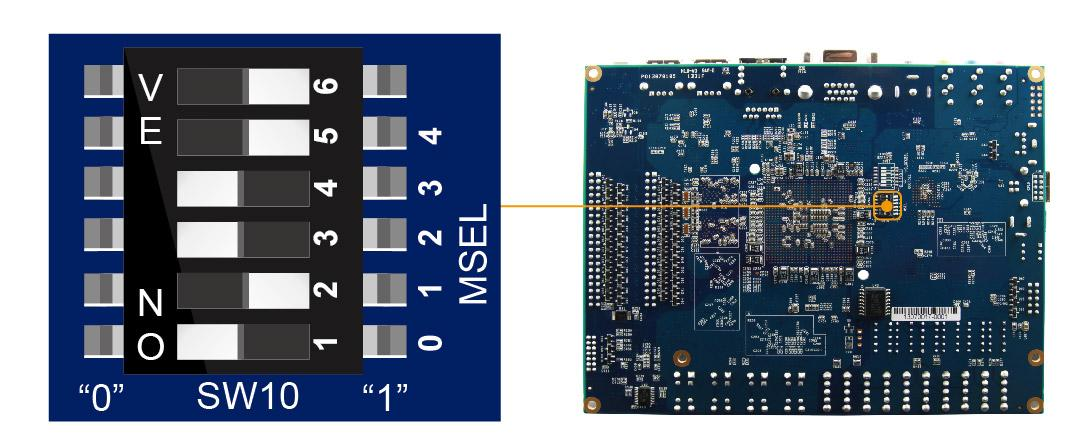
\includegraphics[width=\textwidth]{pictures/msel.png}
\caption{Przełączniki MSEL[0:4] na płytce Terasic DE1-SOC}
\label{fig:msel}
\end{figure}

\begin{figure}[!p]
\centering
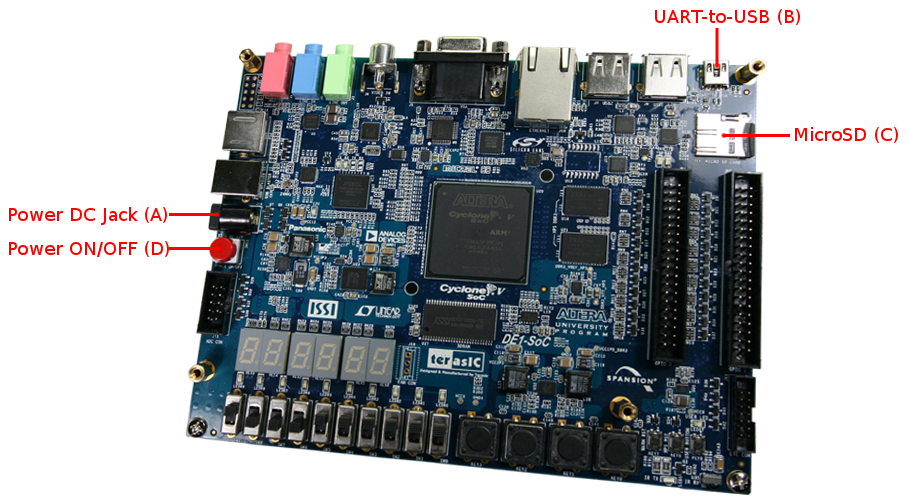
\includegraphics[width=\textwidth]{pictures/fpga-board.jpg}
\caption{Pozycja gniazd na płytce Terasic DE1-SOC}
\label{fig:gniazda}
\end{figure}

\subsection{Instalacja wymaganych bibliotek}
Program komputerowy \textit{fpga-aes} korzysta z interpretera języka python w wersji 2.7, który jest dostarczony z systemem operacyjnym Ubuntu i nie wymaga dodadkowej instalacji. Skrypt korzysta z dodatkowych bibliotek, które można zainstalować następującymi poleceniami:
\begin{interface}{crcmod }
\item[\textbf{serial}] \verb|sudo apt-get install python-serial|
\item[\textbf{crcmod}] \verb|sudo apt-get install python-crcmod|
\end{interface}


